\subsection{29.7.08 - Intravenus de Milo - a diatribe}

 \margininbox{Intravenus de Milo}{
     \begin{itemize}
    \item Clewin Griffiths
    \item James Kirkpatrick
    \end{itemize}}{\explo}

After plenty of trips down \passage{M2}, it was time to push the other side
of the mythical \passage{Gardeners' World}-\passage{M2} connection. James KP
\& I caved down to \passage{Traverse Chamber}, past \passage{Captain
Kangaroo}. Originally I thought that the \passage{Gardeners' World} side
would be more pleasant than \passage{M2}, but then the repressed memories
of \passage{Captain Kangaroo} resurfaced as the passageway turned into a
succession of horrible squeezes, horrible climbs and horrible pitcheads.



Traversing across \passage{Traverse Chamber} and into \passage{Mud Slump}, \bignote{the cave
quality declined somewhat}, decaying into crumbling climbs and pitches
which had been rigged off a dodgy natural, half way down. We pushed on,
hoping to find a PSS with ``\passage{Kill'em All}'' written on it.
Eventually we did. Relief was rapidly followed by shock and despair when
James crawled around the corner and saw the \passage{Kill'em All}
pitchhead. To paraphrase him at the time: ``This is by far and away, and
without a shadow of a doubt the worst and most contemptible pitchead
you'll ever see.'' He wasn't far off. Schematically it looked something
like this: (diagram OKAY DON'T FORGET TO REMOVE THIS FIONA HOPEFULLY THERE WILL BE A DIAGRAM BUT IF NOT) Coming up would certainly be a problem, but we were
going to be exiting via \passage{M2} through the as-yet-undiscovered
connection, so we didn't consider that eventuality.

\begin{marginfigure}
\checkoddpage \ifoddpage \forcerectofloat \else \forceversofloat \fi
\centering
 \frame{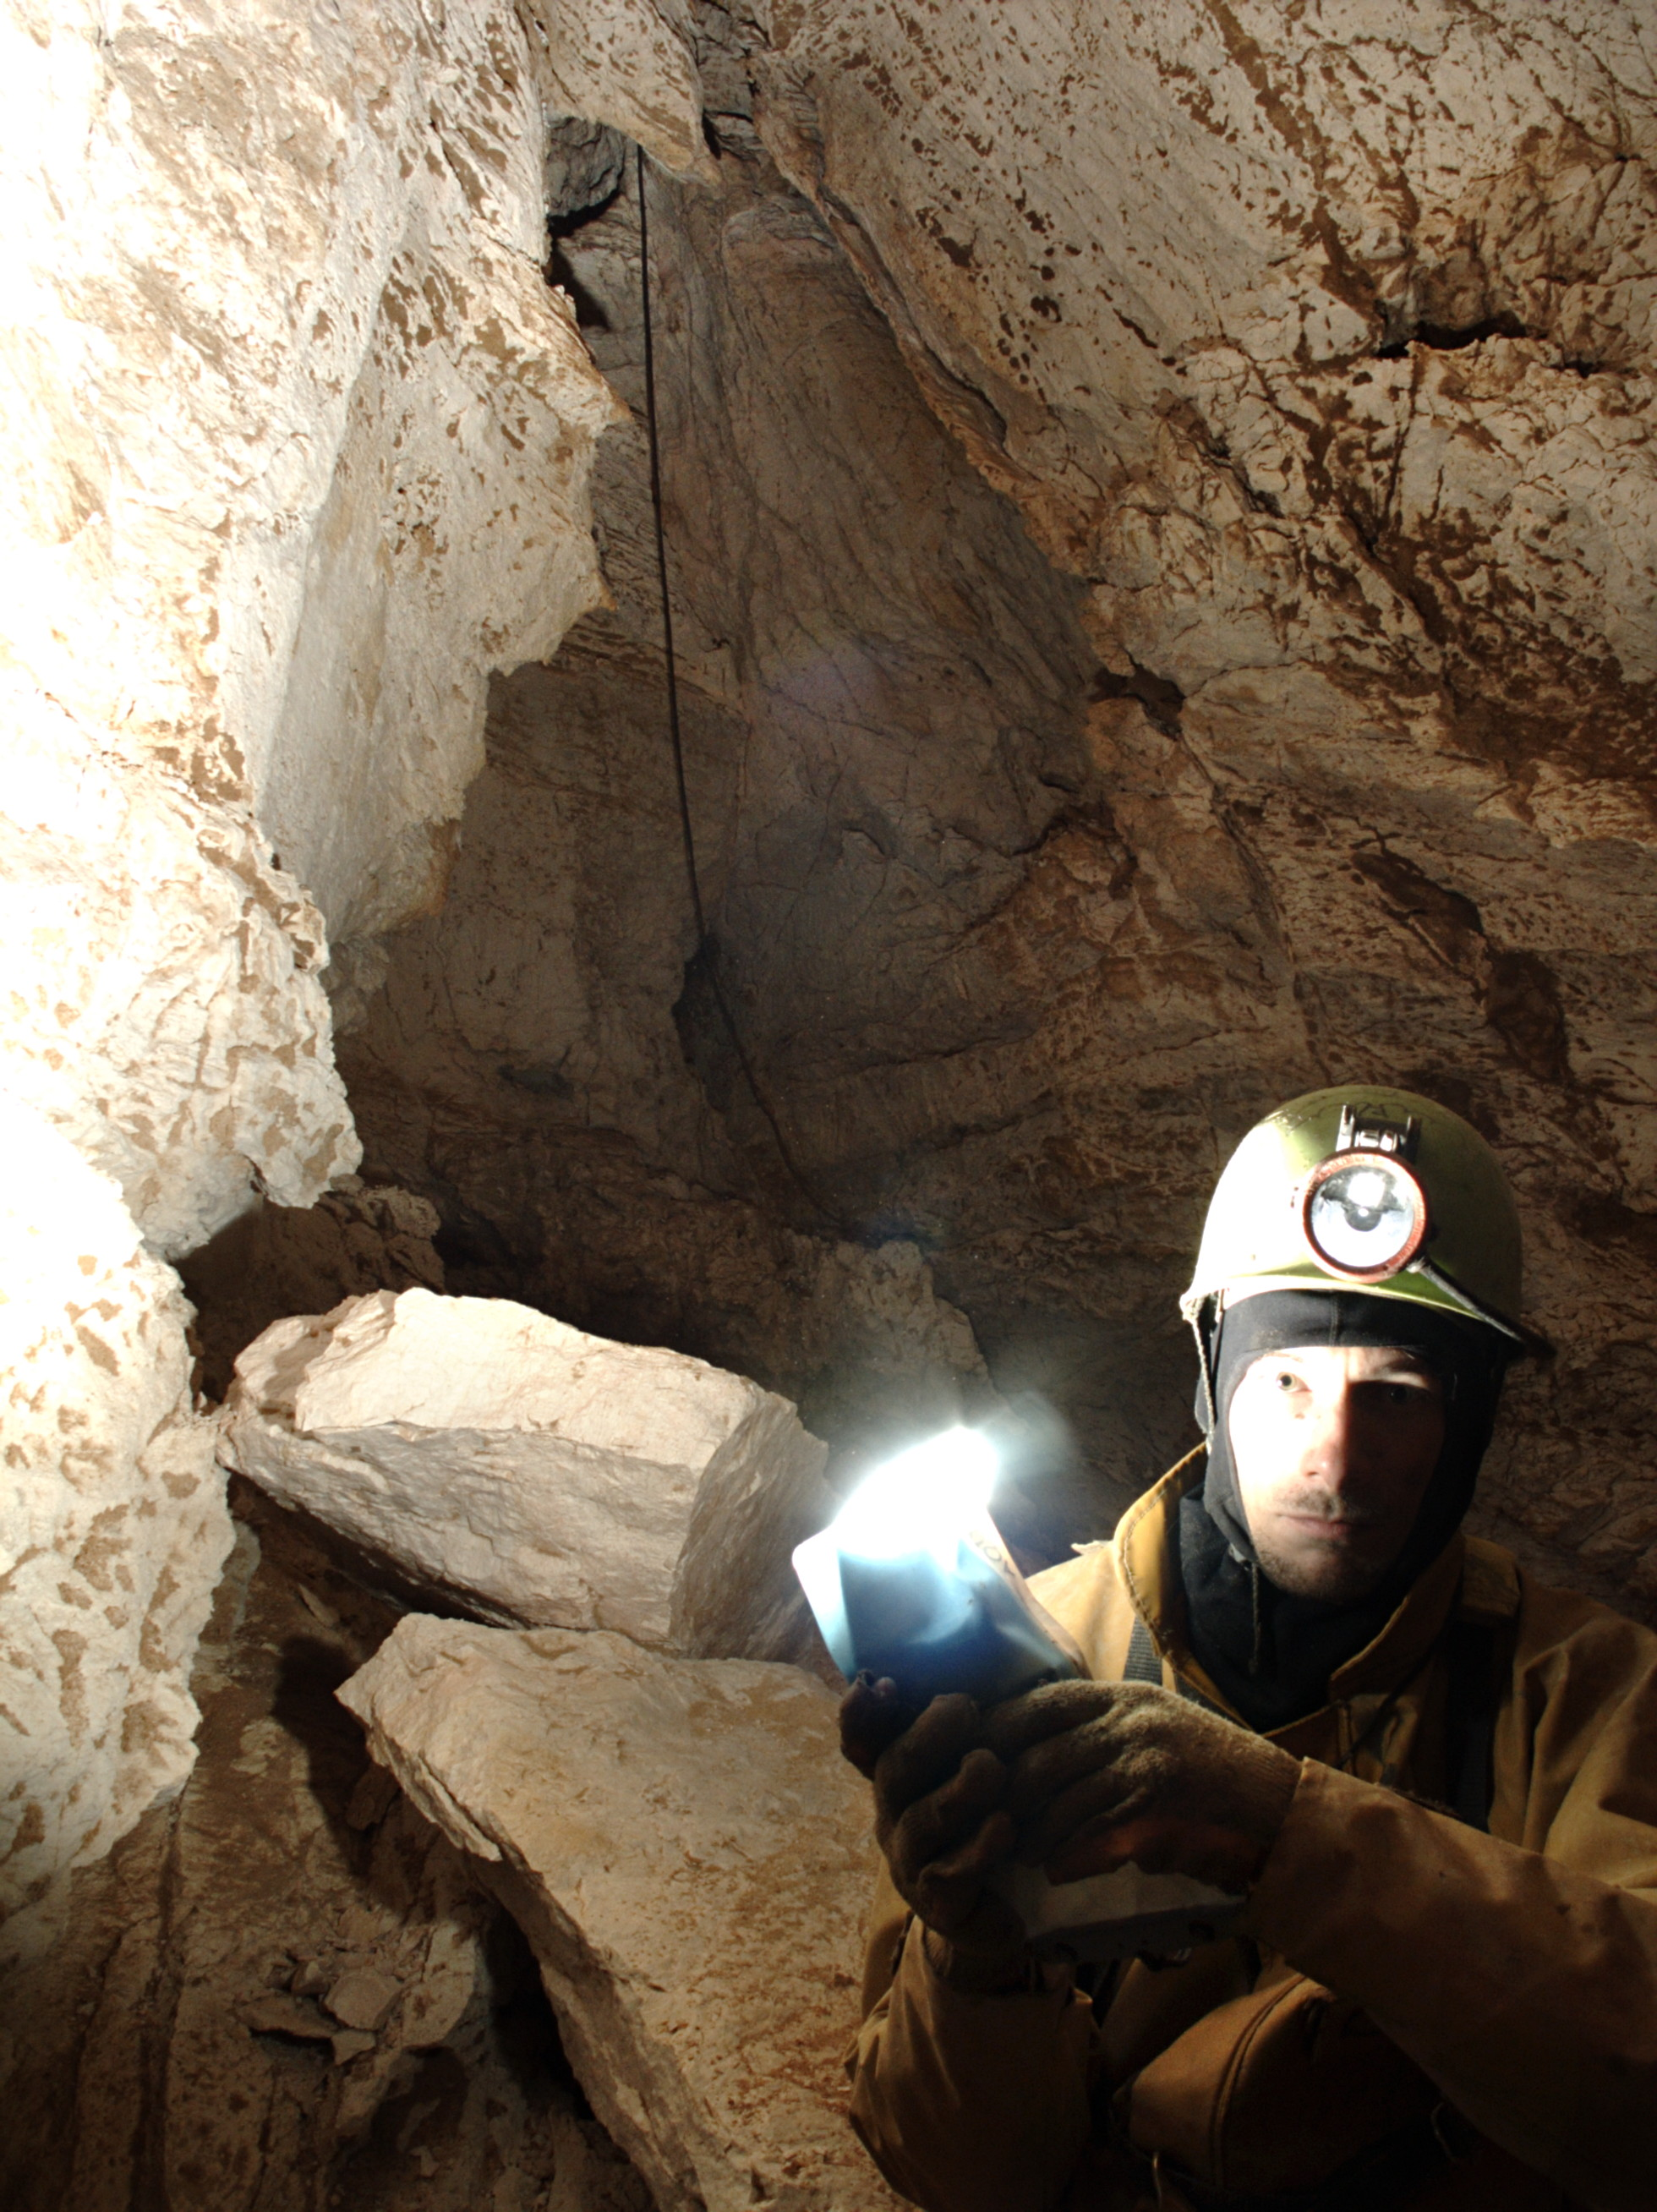
\includegraphics[width=\linewidth]{2008/intravenus/2009-08-10-18.05.38 - Jarvist Frost - Canon Powershot G5 - intravenus de milo chamber - gergely--orig.jpg}} 
 \caption{Gergely Ambrus in \protect\passage{Intravenus de Milo} chamber in 2009. \pic{Jarvist Frost}}
 \label{intravenus chamber}
\end{marginfigure}

Compared with the unspeakable \passage{Mud Slump}, the cave at the bottom of
\passage{Kill'em All} pitch was actually quite nice. There was a climb down
near the bottom of the pitch which we attempted, before the dawning
realisation that rescue after a fall here would be pretty much
impossible. So we rigged off a natural and dropped to the floor. I sat
and smirked as James struggled to get even his helmet through the
miniscule rift at the bottom. So that lead was dead. We derigged and
turned our attention to the only other way on, the rift leading south
from the bottom of the pitch. The rift zigzagged left then right and we
climbed up into a round window on the right.

This lead to a small pitch. I belayed James down and he found a rift at
the bottom leading to a pitch with a ``5 second'' drop. He then revised
that down to 4 sec. I'd suggest 35 m (maybe 2 ½ sec). I put a bolt in
and dropped down so we could survey out.

 \margininbox{Kill'em All 30/31-7}{
     \quote{\textit{The problem wasn’t so much the rigging was bad, as that there was no rigging at all.}}
     \mininame{Jarv, Izi, Paul, James} }{\logbook}

The \passage{Intravenus de Milo} pitch looked really pretty, with horizontal
blades of rock jutting out at various levels. By the time we had
finished surveying, we were running short of time -- 4 hours to our call
out. The way out was fairly desparate, with me getting stuck on climbs
and James stuck in squeezes. No one bit of cave was truly awful, but the
combined effect of 3 solid hours of unrelenting scrot of the purest
variety on the way out started to sap my will to live. Having grit in my
wetsocks grinding away at my toes didn't improve the experience. Still,
got out with 2 mins to go before our callout.

Back in the Bivvy, superb slop and trifle for dessert was really
appreciated. Shockingly, despite my recounting tales of squalor, four
people were eager to go down the next day. Such is the lure of
exploration I guess.

\name{Clewin Griffiths}



(Large multi coloured Grade I of \passage{Mudslump} - \passage{Kill'em All})

James Kirkpatrick's first grade 1 survey: \passage{Dark Tranquillity} Many
curious avens on pitch.

Followed on from \passage{Intravenus de Milo} development. James KP
